\section{Hamiltonian averages}
\subsection{Classical Hamiltonian dynamics}


    \begin{definition}[Phase space coordinates]
    We describe the state of a system of $N$ particles by a tuple 
    $$(q,p)\in \cM^N\times \R^{dN} \defeq \cLs$$
    Where $\cM$ is a $d$-dimensional manifold on which lives the coordinate variable $q$, and $p$ is the momentum coordinate.\\
    The momentum of a particle is its velocity multiplied by its mass, thus we may write 
    $$v=M^{-1}p$$
    where $M$ is a diagonal matrix encoding the masses of each particle, and $v$ is the velocity coordinate.\\
    As we are interested in the evolution of systems through time, we will be considering trajectories through the phase space $\cLs$, functions
    $$\begin{cases}\R_+\mapsto \cLs\\
        t\mapsto (q_t,p_t)
    \end{cases}$$
    \end{definition}
        \begin{definition}[Hamiltonian]
            The Hamiltonian of an atomic system is the function defined on $\cLs$ by\\

            \begin{equation}
                \label{Hamiltonian}
                H(q,p)=\color{blue}{\frac12p^\intercal M^{-1}p}+\color{purple}{V(q)}
            \end{equation}
            
            It is the total energy of the system in state $(q,p)$, sum of its \textcolor{blue}{kinetic energy} and \textcolor{purple}{potential energy}
        \end{definition}

        Using this description, Newton's second law has the following form, which defines Hamiltonian dynamics.

        \begin{equation}
            \label{Hamiltonian dynamics}
            \begin{cases}
                \text d q_t=M^{-1}p_t\dt=\nabla_p H(q_t,p_t)\dt\\
                \text d p_t=-\nabla V(q_t)\dt=-\nabla_q H(q_t,p_t)\dt
            \end{cases}
        \end{equation}


        \begin{remark}
        Equation (\ref{Hamiltonian dynamics}) concisely writes, for $X_t\defeq (q_t,p_t)$, 
        \begin{equation}\label{general hamiltonian equation} \text d X_t=J\nabla H(X_t)\dt\end{equation}
        Where
        $$J=\begin{pmatrix}
            0_{dN} & I_{dN}\\
            -I_{dN} & 0_{dN}
        \end{pmatrix}$$
        is the symplectic matrix. By the chain rule, we have

        \begin{equation}
        \label{conservation of energy} \text d H(X_t)=\text d X_t^{\intercal}\nabla H(X_t)=(J\nabla H(X_t))^\intercal \nabla H(X_t)\dt=0
        \end{equation}
        This relation expresses the fact that the Hamiltonian map is invariant under the flow of equation (\ref{general hamiltonian equation}). This, in turn, is the mathematical translation of the principle of conservation of energy in physics.
        \end{remark}
    
        More generally, we may apply the chain rule to smooth functions $\varphi: \cLs \mapsto \R$.
        We obtain 
        $$ \text d \varphi(X_t)= \text d X_t^{\intercal} \nabla \varphi(X_t)=(J \nabla H(X_t))^\intercal \nabla \varphi(X_t)\dt=(\nabla_p H \cdot \nabla_q - \nabla_q H \cdot \nabla_p)\varphi(X_t)\dt$$

        This motivates the following.
        \begin{definition}[Generator of the Hamiltonian dynamics]
            We define the generator associated with the Hamiltonian dynamics to be the operator $\cL_{\text{H}}$ defined on smooth functions by
        \begin{equation}
            \label{Hamiltonian generator}
            \cL_{\text{H}}\varphi=(\nabla_p H \cdot \nabla_q - \nabla_q H \cdot \nabla_p)\varphi
        \end{equation}
    \end{definition}

    \begin{remark}
        \label{non-separable hamiltonian}
        Property (\ref{conservation of energy}) is only due to the form of $J$, and not to the particular expression for $H$.
        Thus, we may consider any dynamics of the form (\ref{general hamiltonian equation}), to devise a dynamical system whose orbits are restricted to the level set $H^{-1}\{H(q_0,p_0)\}$.\\
        Conversely, given a dynamical system, if through a change of coordinates one is able to write the system under the form (\ref{general hamiltonian equation}), one has found a conservation law.
    \end{remark}

    One key property of the classical Hamiltonian is that it is \textit{separable}: it splits into a kinetic part involving only the momentum variable and a potential part involving only the coordinate variable. We will see when implementing numerical schemes for Hamiltonian systems that separability permits one to construct a number of schemes based on explicit splittings of the evolution operator over a timestep, which turn out to display interesting qualitative properties.
    
        \label{evolution operator exponential notation}

    \subsection{The Lennard-Jones Model}

    \subsection{Numerical integration of Hamiltonian dynamics}
    \subsection{Symplecticity}
    \subsection{Symplectic Euler}
    \subsubsection{Energy conservation properties}
    \begin{figure}[htbp]
        \begin{center}
          \includegraphics[width=0.49\linewidth]{figures/chapter1/energy_fluctuations_SEA.pdf}
          \includegraphics[width=0.49\linewidth]{figures/chapter1/energy_fluctuations_SEB.pdf}
          \caption{ \label{fig:energy_symplectic_euler}
            Absolute variation of the Hamiltonian $ \left\lVert H-\operatorname{min} H\right\rVert_{\infty}$ as a function of the time step over 1000 iterations of the symplectic Euler schemes (A on the left and B on the right). A linear regression line is plotted in red.
          }
        \end{center}
      \end{figure}

    \subsubsection{The Verlet scheme}

    \begin{figure}[htbp]
        \begin{center}
          \includegraphics[width=0.7\linewidth]{figures/chapter1/energy_fluctuations_verlet.pdf}
          \caption{ \label{fig:energy_verlet}
            Absolute variation of the Hamiltonian as a function of the time step over 1000 iterations of the Velocity Verlet scheme. A quadratic regression curve is plotted in red.
          }
        \end{center}
      \end{figure}

    \subsection{Examples of instantaneous observables}
        
    \subsection{Shortcomings of the Hamiltonian approach}

\section{Canonical averages}
    \subsection{The notion of ensemble}

\subsection{Langevin dynamics}
We consider a special case of the inertial Langevin dynamics, defined by the following stochastic differential equation (SDE), where $\gamma, \beta$ are set real constants.

\begin{equation}
    \label{Langevin}
    \begin{cases}
        \text dq_t=M^{-1}p_t\dt \\
        \text dp_t= -\nabla V(q_t)\dt \textcolor{blue}{-\gamma M^{-1}p_t\dt}+\textcolor{purple}{\sqrt{\frac{2\gamma}\beta}\text dW_t}
    \end{cases}
\end{equation}

Where $(W_t)_{t\geq 0}$ is a standard $dN$-dimensional Brownian motion.\\
This process is a combination of a Hamiltonian evolution with an additional action on the momenta which, if isolated, defines a $dN$-dimensional Ornstein-Uhlenbeck process.\\
This additional term be interpreted physically as the combination of two effects: a \textcolor{blue}{dissipation term} which can be understood as the effect of a viscous friction force on the particles, and a \textcolor{purple}{fluctuation term}, which corresponds to the input of kinetic energy into the system as thermal agitation induced by a surrounding heat bath at temperature $1/(k_B\beta)$.\\
However, the physical meaning can be forgotten thanks to the fact that, \textit{in fine}, we only require that the canonical measure be ergodic under this dynamic: as we shall shortly see, this is indeed the case.

\begin{remark}
    There are several ways to generalize this process.\\
    One way is to consider more general, possibly non-separable, Hamiltonians, as in (\ref{non-separable hamiltonian}), rather than the classical Hamiltonian used above.\\
    The other is to allow the fluctuation-dissipation term to be parametrized by coefficients $\gamma$ and $\sigma$ depending on the state variable, and which obey a relation ensuring ergodicity.\\
    Hence in full generality, we could consider the following Langevin dynamic:
    
    \begin{equation}
        \label{general Langevin}
        \begin{cases}
            \text dq_t=\nabla_p H(q_t,p_t)\dt \\
            \text dp_t= -\nabla_q H(q_t,p_t)\dt -\gamma(q_t,p_t)\nabla_pH(q_t,p_t)\dt+\sigma(q_t,p_t)\text dW_t
        \end{cases}
    \end{equation}
\end{remark}



\subsection{Properties of the Langevin dynamics}

To investigate some of the properties of the dynamics, it is useful to introduce the notion of a generator for a process defined by a possibly inhomogeneous SDE.
\subsubsection{The generator}
We consider a general process defined by a SDE of the form:

\begin{equation}
    \label{SDE}
    \text dX_t=b(t,X_t)\text \dt + \sigma(t,X_t)\text dW_t
\end{equation}

Where $b$ is a $\R^n$-valued function, $W$ is a standard $d$-dimensional Brownian motion and $\sigma$ is a $n\times d$ matrix-valued function.\\
For $\varphi$ a smooth bounded function, Itô's lemma allows us to compute:
\begin{align*}
    d\varphi(t,X_t) &=\frac{\partial \varphi}{\partial t}(t,X_t)\text dt + \nabla^\intercal \varphi(t,X_t) \text dX_t + \frac12 \operatorname{Tr}(\nabla^{2\intercal}\varphi(t,X_t)\text d\langle X ,X\rangle _t)\\
    &=\left( \frac{\partial \varphi}{\partial t} + \nabla^{\intercal}\varphi b + \frac12 \operatorname{Tr}(\nabla^2\varphi \sigma\sigma^\intercal) \right)(t,X_t) \text dt+ (\nabla^\intercal \varphi\sigma )(t,X_t)\text dW_t
\end{align*}

Where $\nabla$, $\nabla^2$ are with respect to the spatial coordinates. In other words,\\


\begin{equation}
    \label{Ito}
    \varphi(t,X_t)= \varphi(0,X_0)+\int_0^t\left( \frac{\partial \varphi}{\partial t} + \nabla^\intercal\varphi b + \frac12 \operatorname{Tr}(\nabla^2\varphi\sigma\sigma^\intercal) \right)(s,X_s) \text ds + \int_0^t\nabla^\intercal \varphi\sigma(s,X_s)\text dW_s
\end{equation}
%----invariance of $\mu$

    \begin{definition}[Generator of an Itô process]
        Let $X_t$ be a $\R^n$-valued process defined by \ref{SDE}. We define its generator at time $t$ as the operator defined by

        \begin{equation}
            \label{Generator}
            \cL_t \varphi(x)=\left(\frac{\partial \varphi}{\partial t} + \nabla^\intercal\varphi b + \frac12 \operatorname{Tr}(\nabla^2\varphi \sigma\sigma^\intercal)\right)(t,x)
        \end{equation}

    \end{definition}

    In view of (\ref{Ito}), we have, provided regularity conditions on $\sigma$ and $\varphi$,
    $$\E\left[\varphi(t,X_t)\right|X_s=x]=x+\int_s^t \E[\cL_u\varphi(X_u)] \text du$$
    so that, at least formally,
    \begin{equation}
    \label{generator formal motivation}
    \frac{\partial}{\partial t}\E[\varphi(t,X_t) | X_{s}=x]=\E[\cL_{t} \varphi(X_{t})|X_{s}=x]=\cL_{t}\E[\varphi(t,X_{t})|X_{s}=x]
    \end{equation}

    If we define a family of evolution operators $(P_{s,t})_{s\leq t}$ by the formula
    $$P_{s,t} \varphi (x)= \E[ \varphi (t,X_t) | X_s=x] $$
    (\ref{generator formal motivation}) rewrites
    $$ \frac{\partial}{\partial t} P_{s,t} \varphi (x)=P_{s,t}\cL_t\varphi(x)=\cL_t P_{s,t}\varphi(x)$$
    
    An important special case occurs when $b,\ \sigma$ and $\varphi$ do not depend on time. In this case the generator is a single operator $\cL$, defined by
    $$\cL \varphi = \nabla^\intercal \varphi b + \frac12 \operatorname{Tr}(\nabla^2 \varphi \sigma \sigma ^\intercal)$$ 
    The evolution operators $P_t \defeq P_{0,t}$ ($ = P_{s,s+t}\ \forall s$ by stationarity) form a semi-group, and act on the space of smooth functions as
    $$ P_t \varphi(x)= \E[\varphi(X_t)| X_0=x]$$
    The formal derivative is given by
    $$ \frac{\partial}{\partial t}P_t=P_t\cL=\cL P_t$$
    
    As in (\ref{evolution operator exponential notation}), we may write, by analogy with the finite-dimensional setting,
    $e^{t\cL}\defeq P_t$


    \subsubsection{Invariance of the canonical measure}

    The Langevin dynamics (\ref{Langevin}), when written under the form (\ref{SDE}), corresponds to the case 

    $$ b(q,p)= \begin{pmatrix} M^{-1}p \\ -
    \nabla V(q)-\gamma M^{-1}p\end{pmatrix},\ \sigma(q,p)= \sqrt{\frac{2\gamma}\beta}\begin{pmatrix} 0_{dN} &  0_{dN} \\  0_{dN} & \text{I}_{dN} \end{pmatrix}$$
    Hence, applying \ref{Generator}, we obtain the generator for the dynamics
    $$ \cL=  \cL_q + \cL_p $$
    where
    $$ \cL_q \varphi= \nabla^\intercal_q\varphi M^{-1}p$$
    $$ \cL_p\varphi =-\nabla^\intercal_{p}\varphi (\nabla V(q)+\gamma M^{-1}p) +\frac{\gamma}{\beta}\Delta_p $$
    which we may rewrite, recognizing the generator for the Hamiltonian dynamics \ref{Hamiltonian generator}
    $$ \cL=\cL_{H}+\gamma \cL_{\text{ou}}$$
    where $\cL_{\text{ou}}\varphi =-M^{-1}\nabla^\intercal_p\varphi p + \frac1{\beta}\Delta_p\varphi$

    \begin{lemma}
        Let $\varphi,\psi$ be smooth compactly supported functions on $\cLs$. Then
    \end{lemma}

\subsection{Numerical integration of the Langevin dynamics}
text
    \subsubsection{Splitting methods}
    text
    \subsubsection{Implementation}
    text
    \begin{figure}[htbp]
        \begin{center}
            \includegraphics[width=0.49\linewidth]{figures/chapter1/velocities_20.pdf}
            \includegraphics[width=0.49\linewidth]{figures/chapter1/velocities_200.pdf}
            \includegraphics[width=0.49\linewidth]{figures/chapter1/velocities_400.pdf}
            \includegraphics[width=0.49\linewidth]{figures/chapter1/velocities_1000.pdf}
          \caption{ \label{fig:velocity_histograms}
            Convergence of the velocity distribution to a mixture of Maxwell-Boltzmann distributions for a mixture of two ideal gases with different atomic masses, starting from a Dirac distribution $\delta_{\sqrt 3}$. Snapshots of the empirical distribution are shown after 20,\ 200,\ 400 and 1000 steps ($\dt=5\times 10^{-3} \tau ^*, T=T^*$)          }
        \end{center}
      \end{figure}


\subsection{Illustration: the equation of state of Argon}
text
\begin{figure}[htbp]
    \begin{center}
      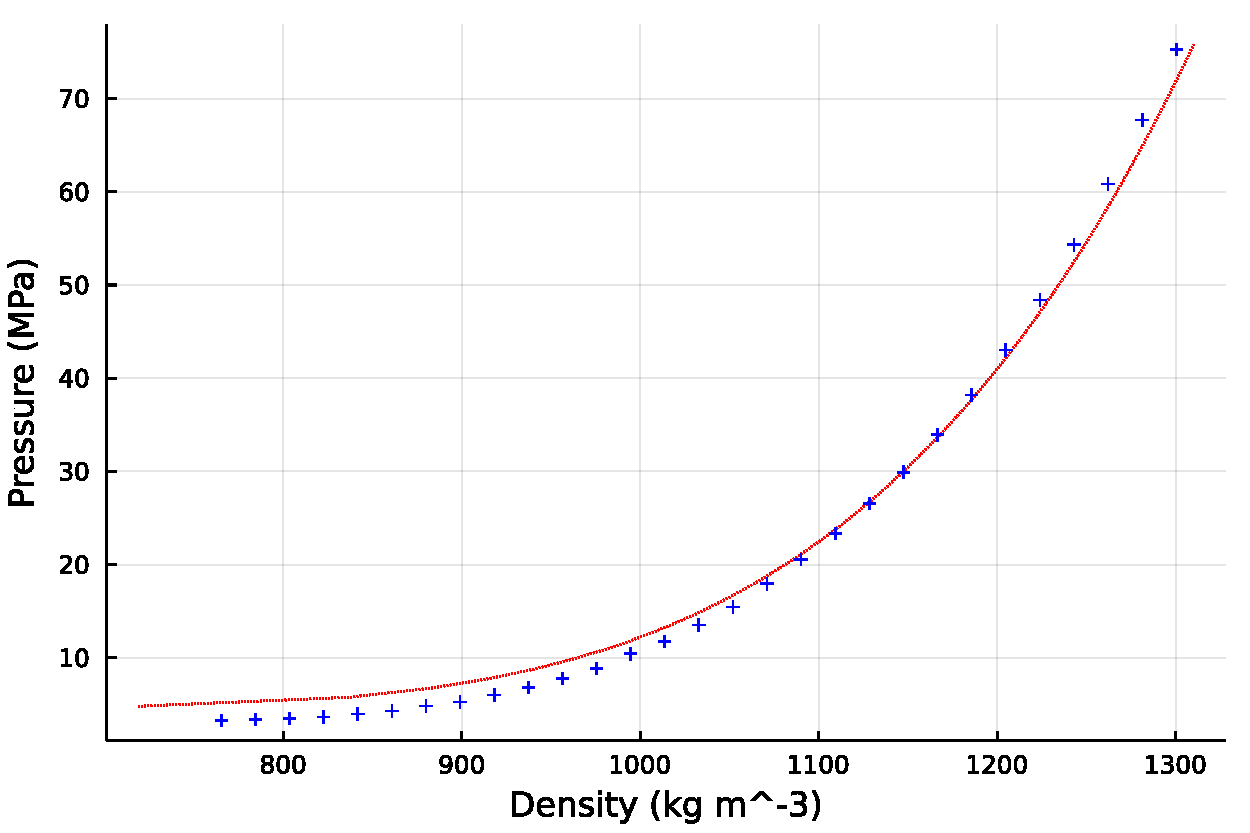
\includegraphics[width=0.49\linewidth]{figures/chapter1/argon_150K.pdf}
      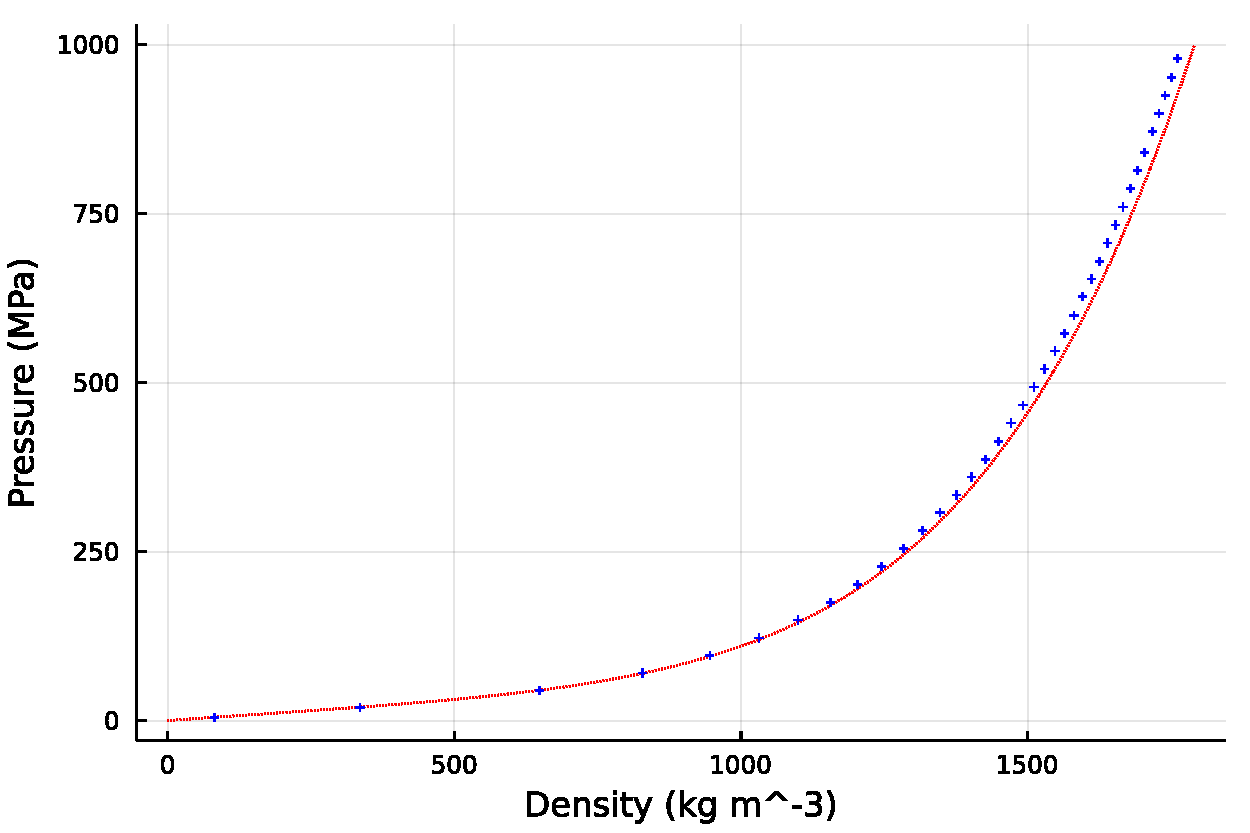
\includegraphics[width=0.49\linewidth]{figures/chapter1/argon_300K_sparse.pdf}
      \caption{ \label{fig:eos_argon}
        Simulated equations of state of Argon at 150 K (liquid phase) on the left and 300K (supercritical phase) on the right. Simulated data points are shown in blue, and the red dotted curve shows the results of experimental measurements.
      }
    \end{center}
  \end{figure}
\subsection{The Metropolis method}